\documentclass{beamer}
\usetheme{CambridgeUS}
\usecolortheme{default}
\setbeamercolor{itemize item}{fg=darkred!80!black}

\makeatletter
\setbeamertemplate{footline}
{
  \leavevmode%
  \hbox{%
  \begin{beamercolorbox}[wd=.333333\paperwidth,ht=2.25ex,dp=1ex,center]{author in head/foot}%
    \usebeamerfont{author in head/foot}F. Massa
  \end{beamercolorbox}%
  \begin{beamercolorbox}[wd=.333333\paperwidth,ht=2.25ex,dp=1ex,center]{title in head/foot}%
    \usebeamerfont{title in head/foot}Supervisors: G. Chiarelli, C. Gemme
  \end{beamercolorbox}%
  \begin{beamercolorbox}[wd=.333333\paperwidth,ht=2.25ex,dp=1ex,right]{date in head/foot}%
    \usebeamerfont{date in head/foot}\insertshortdate{}\hspace*{2em}
    \insertframenumber{} / \inserttotalframenumber\hspace*{2ex} 
  \end{beamercolorbox}}%
  \vskip0pt%
}
\makeatother

\title{ITk performances in the
$H \rightarrow ZZ^{*} \rightarrow 4\mu$ channel \\
with a fast sim method}
%\subtitle{Subtitle}
\author{Federico Massa}
\institute{ITk Simulation \& Performance}
\date{Sept. 7, 2016}

\usepackage[export]{adjustbox}
\usepackage{tikz}
\usetikzlibrary{decorations.pathreplacing,calc}
\newcommand{\tikzmark}[1]{\tikz[overlay,remember picture] \node (#1) {};}

\usepackage{xcolor}
\definecolor{dred}{RGB}{200,0,0}

\usepackage[font=small,skip=0pt]{caption}
\usepackage{textcomp}

\setbeamertemplate{navigation symbols}{}
\begin{document}

\begin{frame}
\titlepage
\end{frame}

%----------------------------------------------

\begin{frame}
\frametitle{Layouts}
\begin{columns}
\begin{column}{0.5\textwidth}
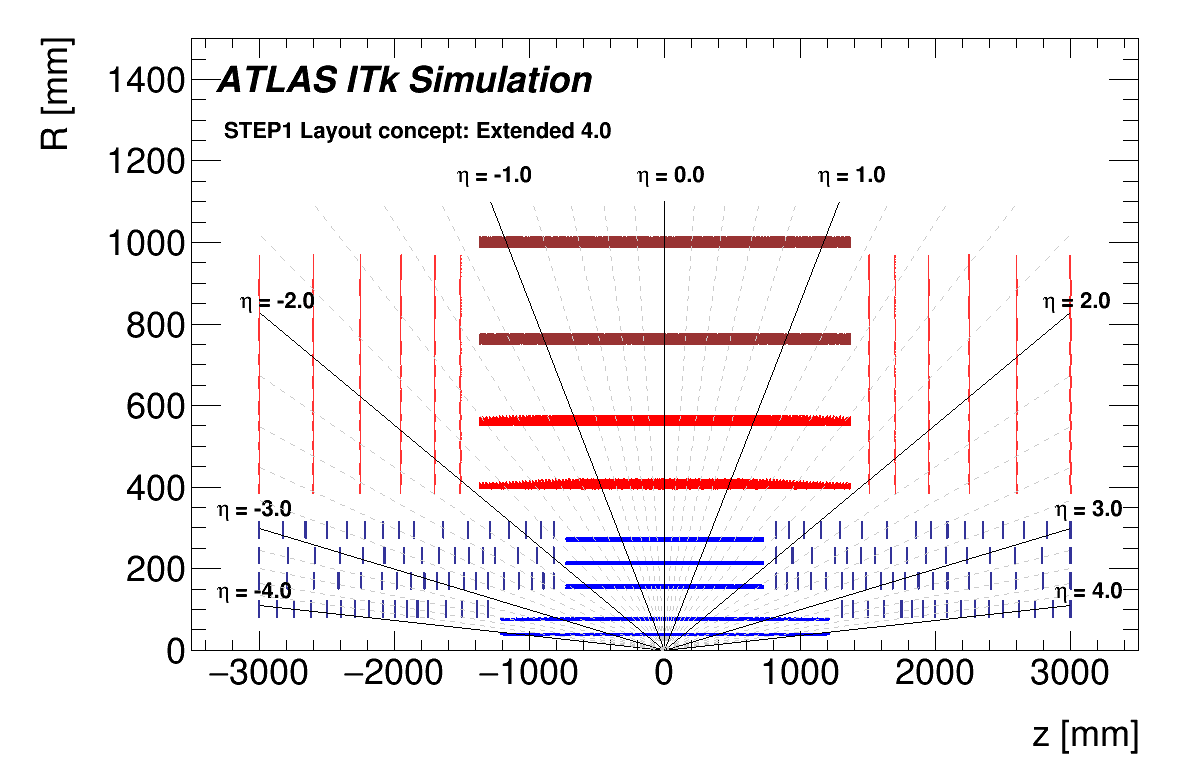
\includegraphics[width=\textwidth,height=3.8cm]{ExtBrl4}
\end{column}
\begin{column}{0.5\textwidth}
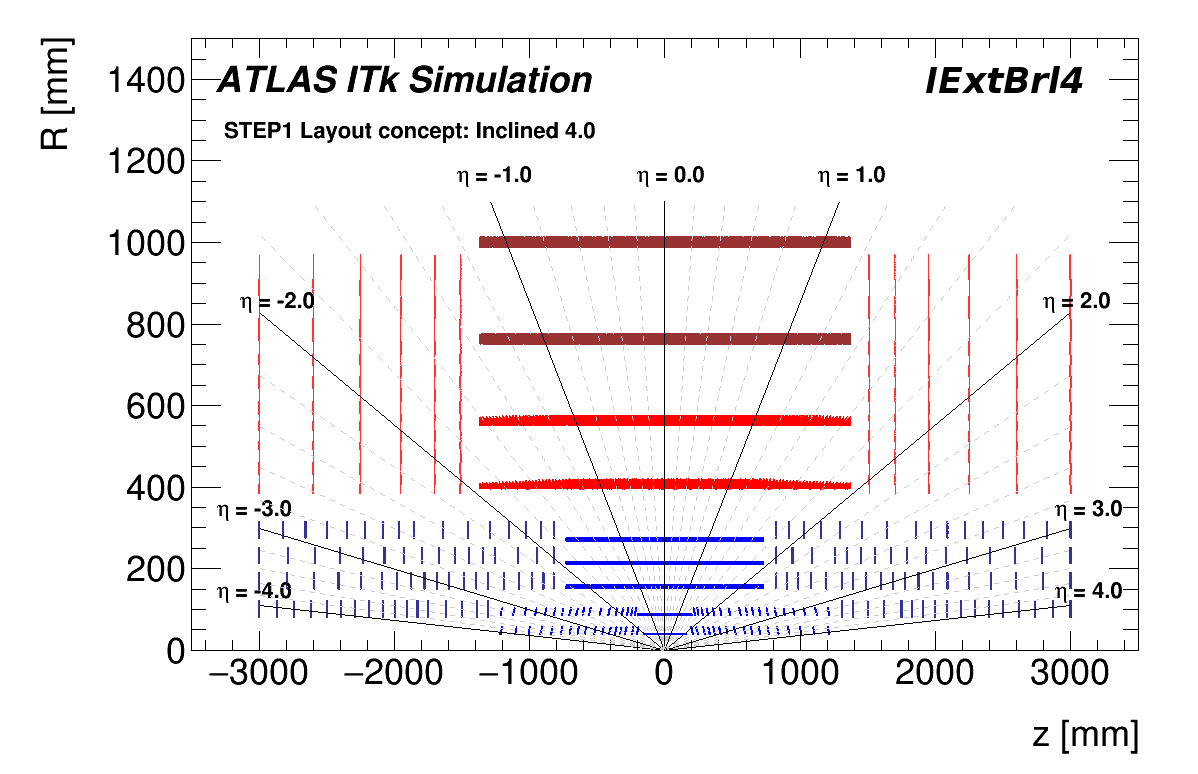
\includegraphics[width=\textwidth,height=3.8cm]{IExtBrl4}
\end{column}
\end{columns}

\begin{columns}
\begin{column}{0.5\textwidth}
\begin{itemize}
\item Step 1 layouts
\item Release 20.20.0.1
\item ExtBrl4 not optimized for long clusters
\end{itemize}
\end{column}
\begin{column}{0.5\textwidth}
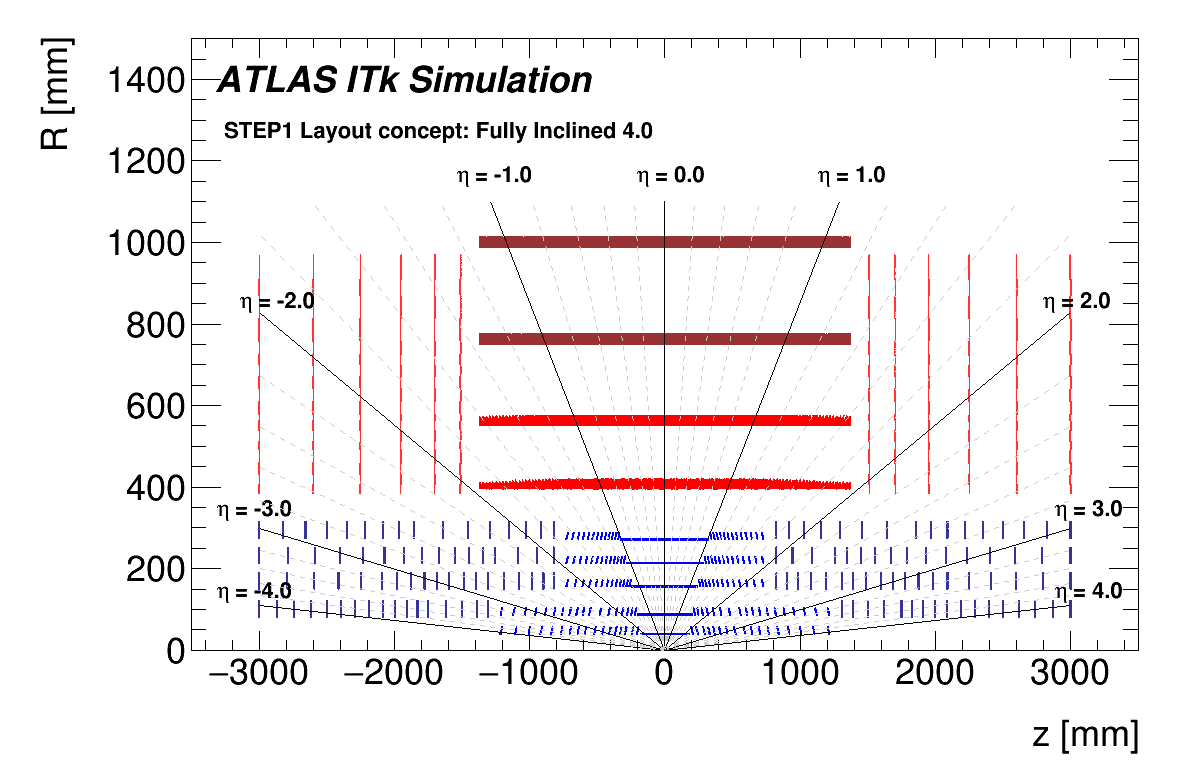
\includegraphics[width=\textwidth,height=3.8cm]{InclBrl4}
\end{column}
\end{columns}

\end{frame}

%----------------------------------------------

\begin{frame}
\frametitle{The Fast Sim method - RoI definition}

\begin{columns}[t]
	\begin{column}{.7\textwidth}
		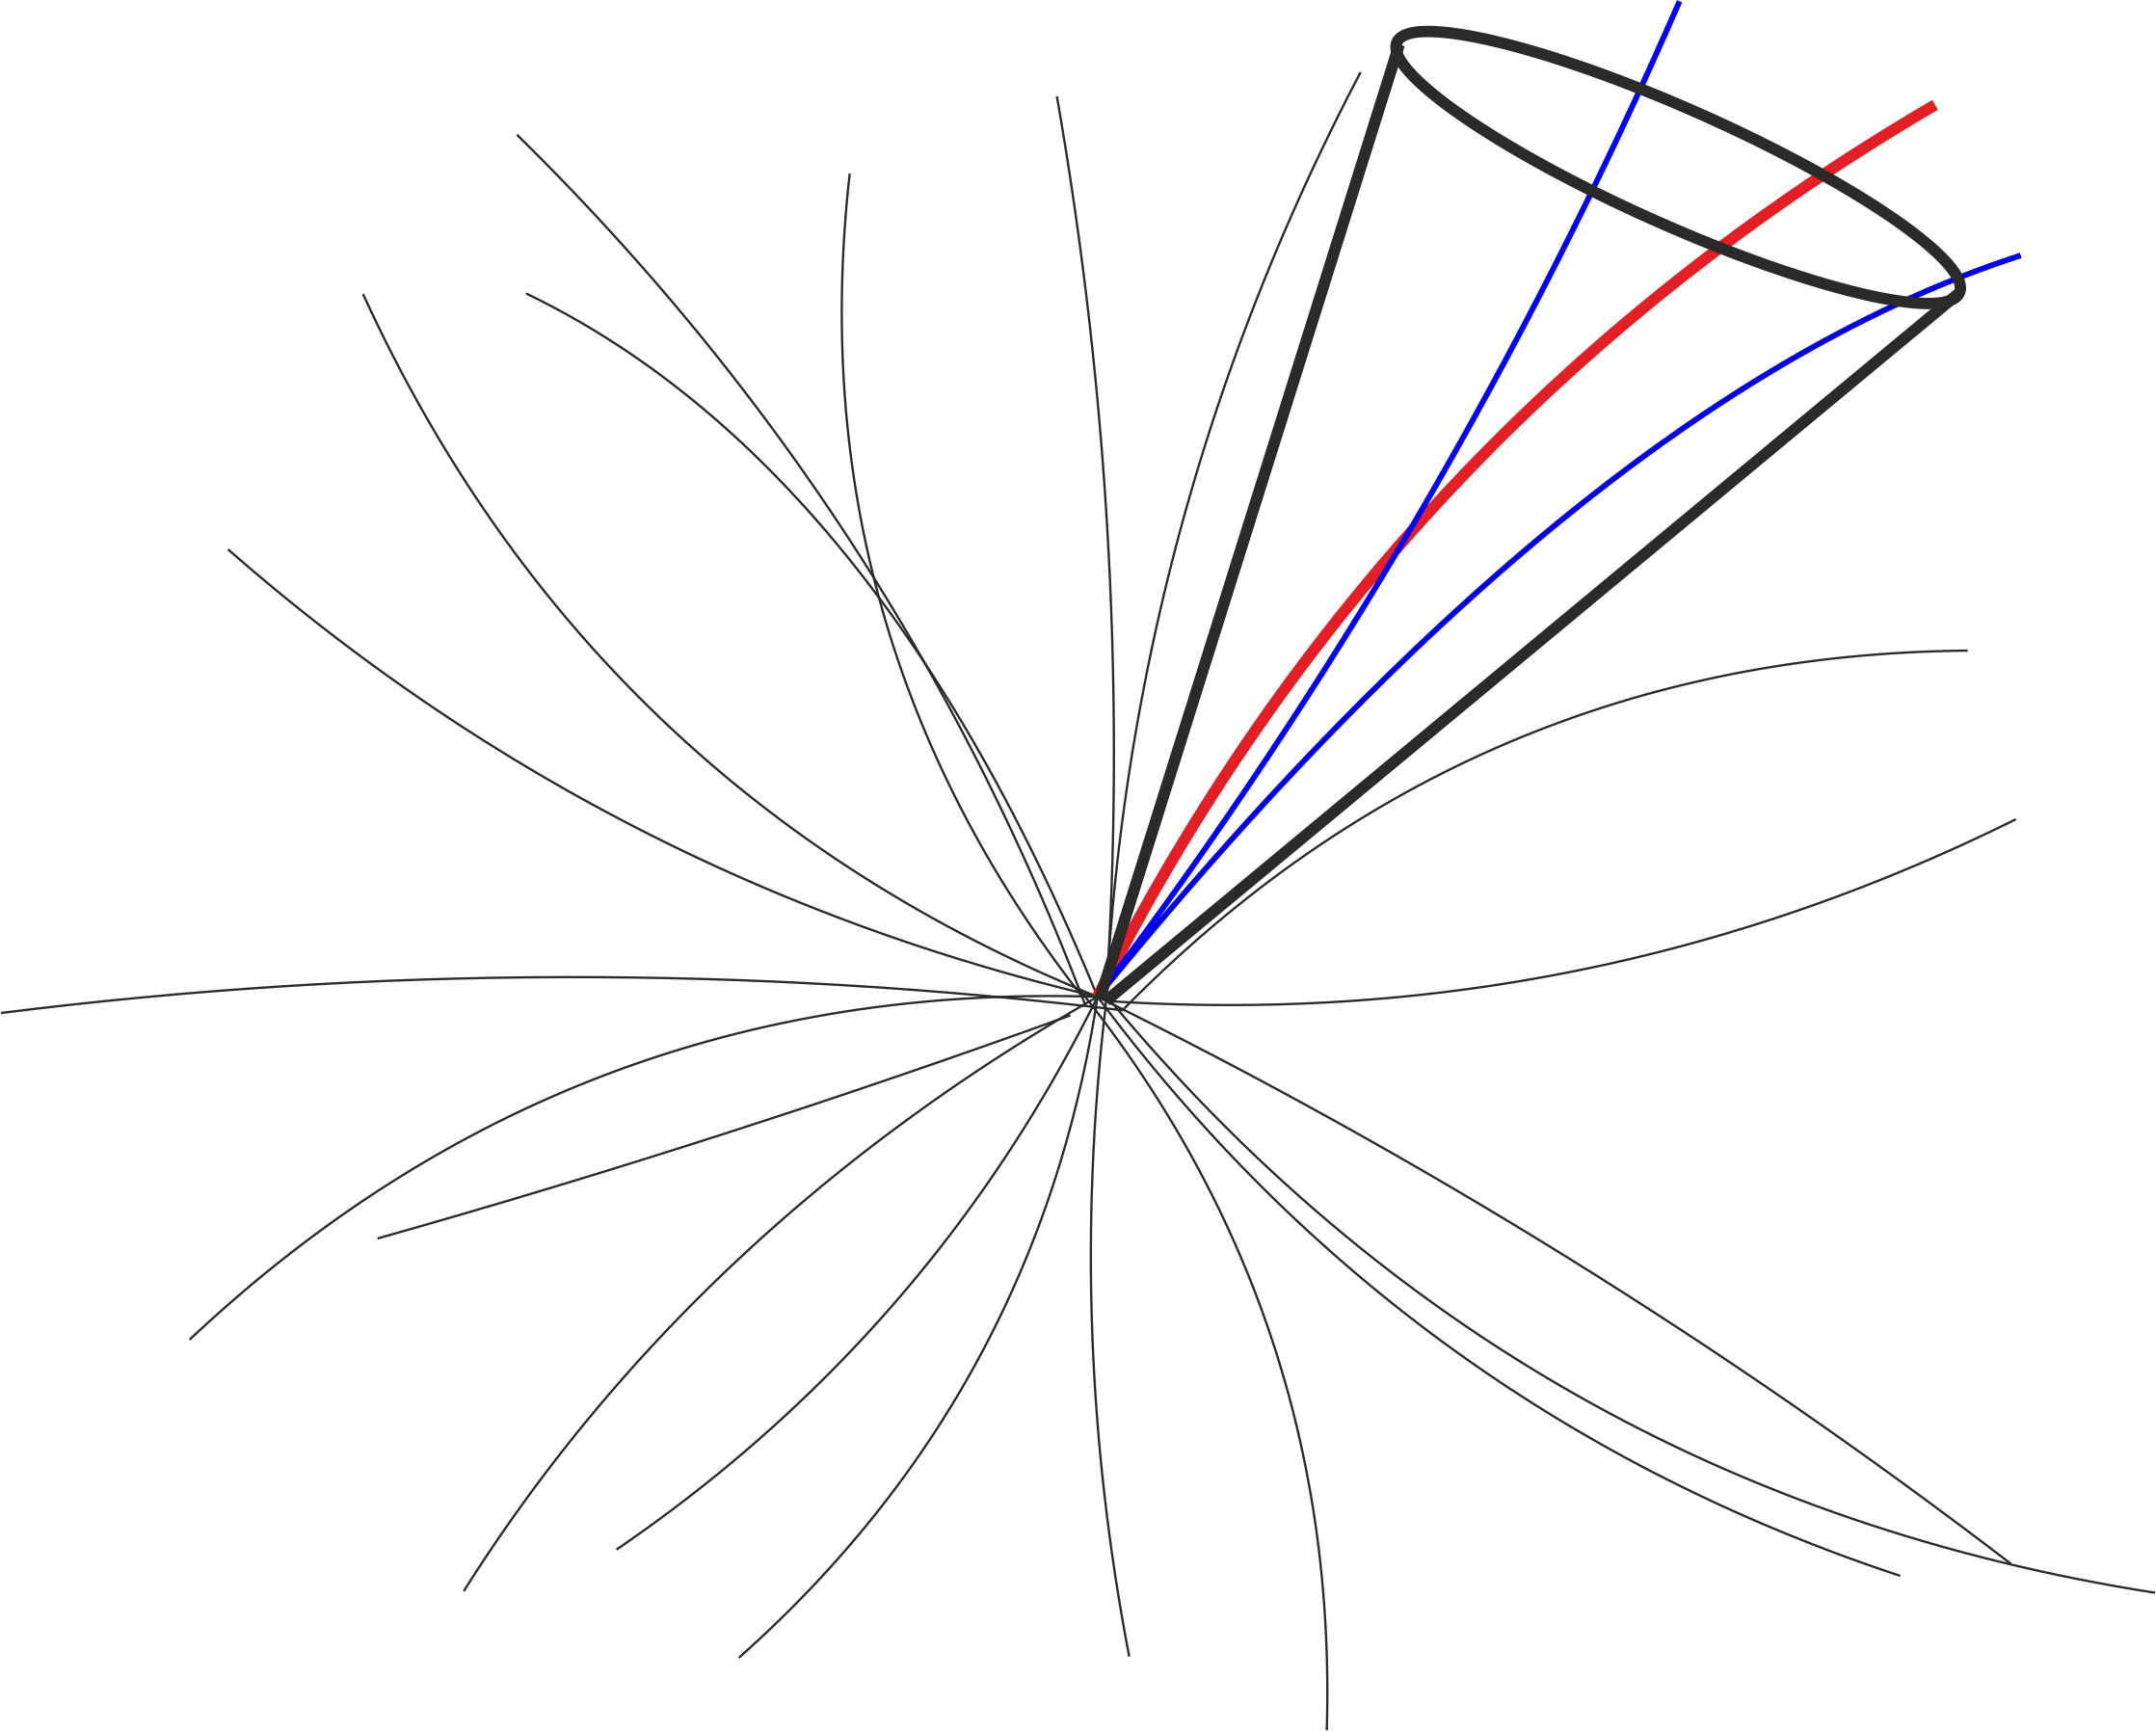
\includegraphics[width=\textwidth,valign=T]{cone}
	\end{column}
	\begin{column}{.3\textwidth}
		
		\small
		{\color{red} Hard-scattering particle} \\
		\vskip0.8cm
		{\color{cyan} Pile-up particles in RoI} \\
		\vskip0.8cm
		{\color{gray} Pile-up particles outside RoI} \\
		\vskip1.5cm
		\framebox{Cone $\Delta$R = 0.1}
	\end{column}
\end{columns}
	
\end{frame}

%----------------------------------------------

\begin{frame}[t]
\frametitle{The Fast Sim method - Algorithm}

\only<1>{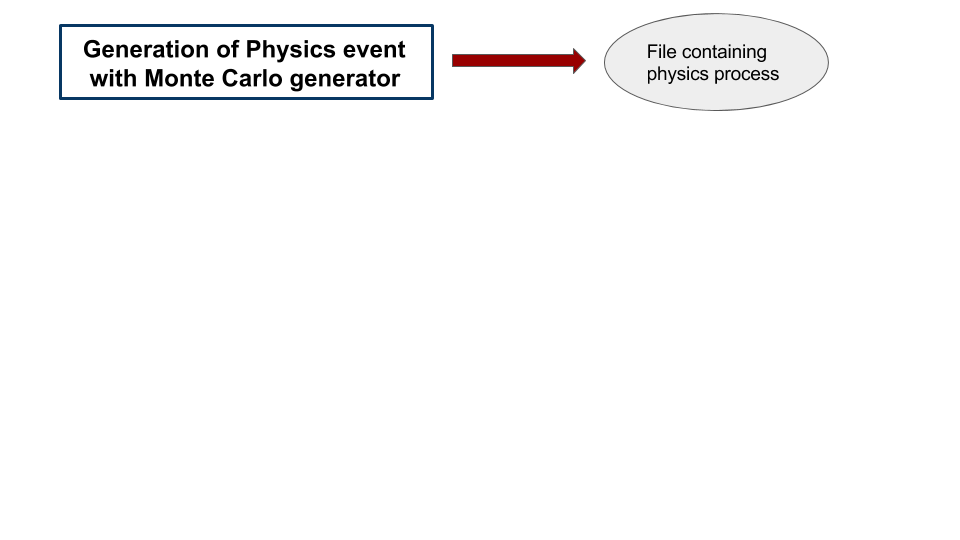
\includegraphics[width=\textwidth]{PhysicsGenerationFlow_1}}
\only<2>{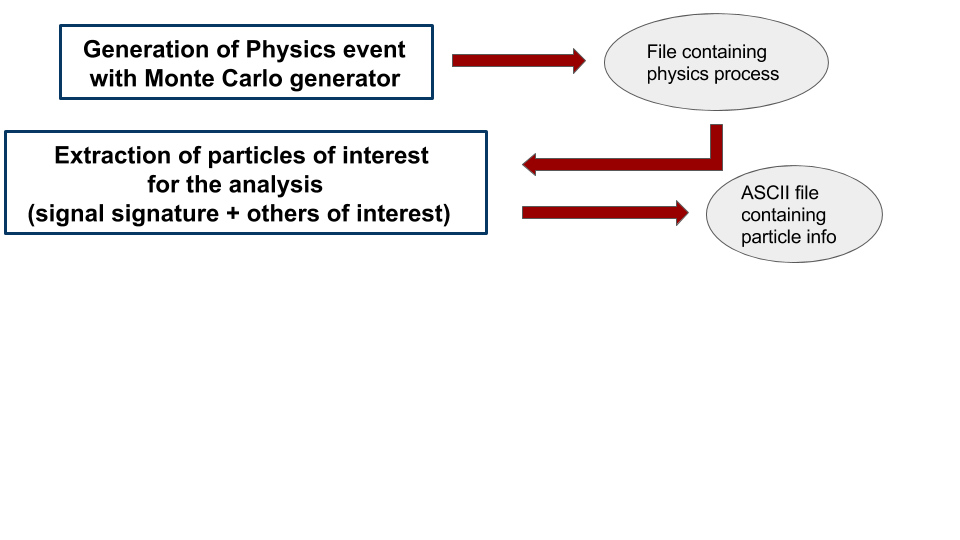
\includegraphics[width=\textwidth]{PhysicsGenerationFlow_2}}
\only<3>{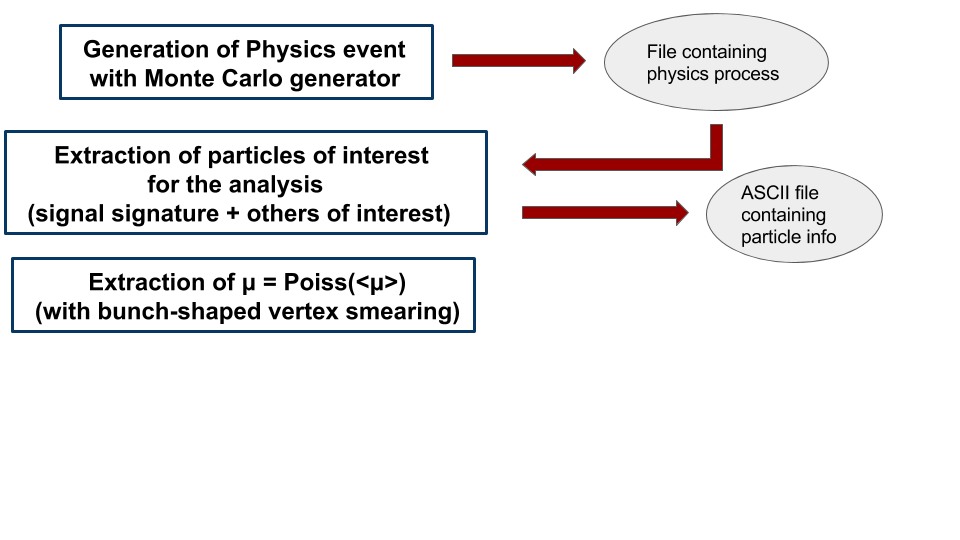
\includegraphics[width=\textwidth]{PhysicsGenerationFlow_3}}
\only<4>{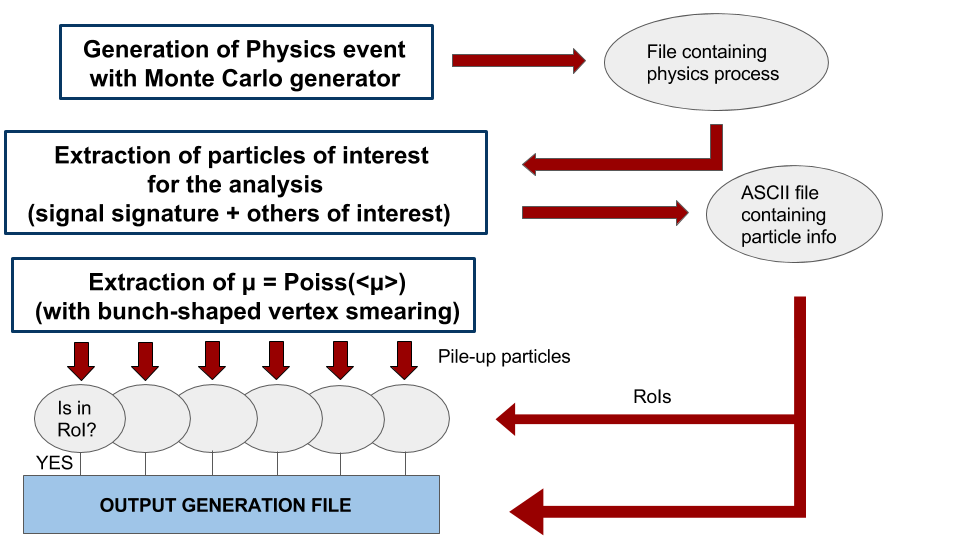
\includegraphics[width=\textwidth]{PhysicsGenerationFlow_4}}

\end{frame}

%----------------------------------------------

\begin{frame}[t]
\frametitle{Generated events}

\begin{itemize}
\item 50k events of $gg\rightarrow H \rightarrow ZZ^{*} \rightarrow 4\mu$ (signal) \tikzmark{topbrace}
\item 16k events of $ZZ^{(*)} \rightarrow 4\mu$ (background) \tikzmark{bottombrace}
\end{itemize}

\setbeamercolor{local structure}{fg=dred} 
\begin{itemize}
\item $\langle\mu\rangle$ = 200, 13 TeV, Step-1 layouts @4.0
\item only events with exactly four muons and $\gamma$ with $p_{T, max}^{\gamma} < 1.5$ GeV
\end{itemize}
%[\color{red}\scalebox{0.9}{\ball}]
\begin{tikzpicture}[overlay, remember picture]
\draw [decoration={brace,amplitude=0.5em},decorate,ultra thick,black]
let \p1=(topbrace), \p2=(bottombrace) in
({max(\x1,\x2)}, {\y1+0.8em}) -- node[right=0.6em] {POWHEG} ({max(\x1,\x2)}, {\y2});
\end{tikzpicture}
%

\begin{columns}
\begin{column}{.5\textwidth}
\centering
Truth $4\mu$ mass in $ZZ^{(*)} \rightarrow 4\mu$
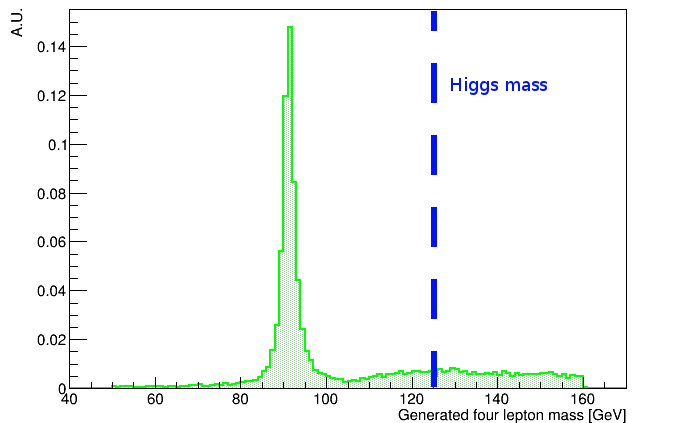
\includegraphics[width=\textwidth]{ZZ4mu/gen4muMass4}
\end{column}
\begin{column}{.5\textwidth}
\centering
Photon $p_{T}$\par
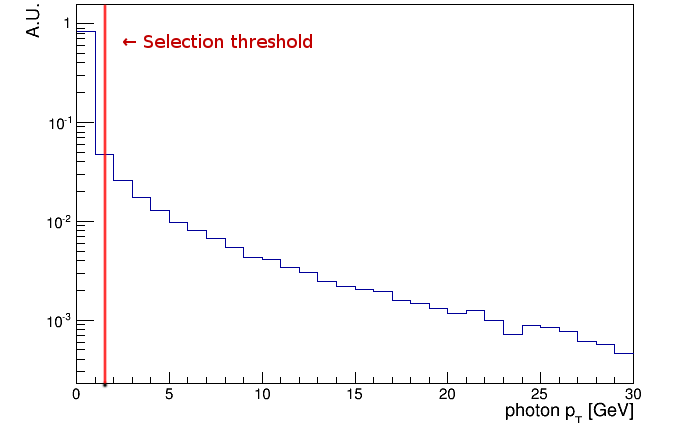
\includegraphics[width=\textwidth]{HZZ4mu/photonPt4}
\end{column}
\end{columns}
\end{frame}

%----------------------------------------------

\begin{frame}
\frametitle{Truth Z mass distribution}

\begin{columns}
\begin{column}{.5\textwidth}
\centering
$H \rightarrow ZZ^* \rightarrow 4\mu$
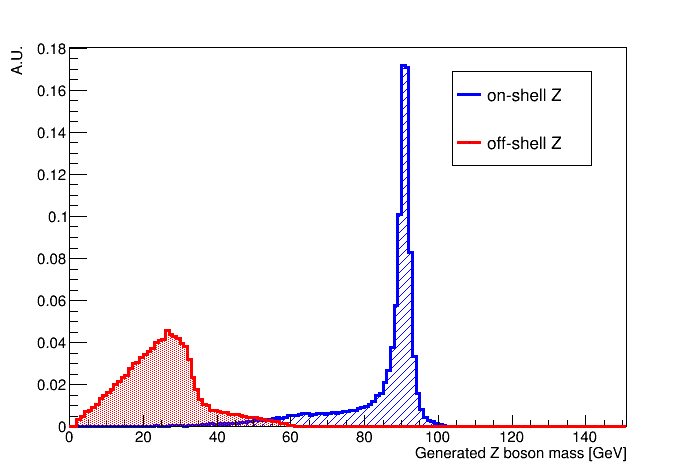
\includegraphics[width=\textwidth]{HZZ4mu/genZMass}
\end{column}
\begin{column}{.5\textwidth}
\centering
$ZZ^{(*)} \rightarrow 4\mu$\par
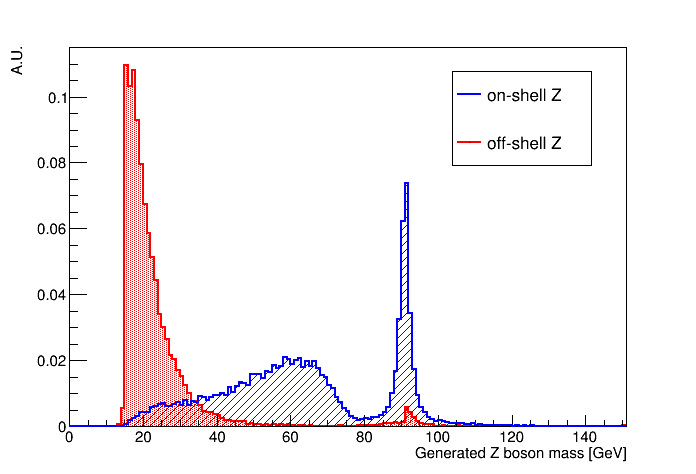
\includegraphics[width=\textwidth]{ZZ4mu/genZMass}
\end{column}
\end{columns}
\end{frame}

%----------------------------------------------

\begin{frame}[t]
\frametitle{Analysis selection}

Requirements are applied in sequence:
\begin{itemize}
\item<1-> at least four tracks in the event;
\item<2-> tracks must consist of at least 10 hits;
\item<3-> tracks must have $p_{T} >$ 6 GeV;
\item<4-> tracks should be closer than 5$\sigma_{z}$ to the truth primary vertex;
\end{itemize}
\medskip
\pause
\pause
\pause
\pause
At this point, all events contain no more than four tracks:
\begin{itemize}
\item<6-> tracks should be isolated: $\sum_{\Delta R < 0.1} (p_{T}) / p_{T, candidate} <$ 1;
\item<7-> the system must be electrically neutral;
\item<8-> the ordered $p_{T}$ of the tracks must be ($>$ 20, $>$ 15, $>$10, $>$ 6) GeV;
\item<9-> at least one of the off-shell candidates (neutral pair with most distant mass from the Z)
must lie in the region $|\eta| <$ 2.7;
\item<10-> the mass of the on-shell pair should lie in the region [50,106] GeV;
\item<11-> the mass of the off-shell pair should lie in the region [12,115] GeV;
\end{itemize}

\end{frame}

%----------------------------------------------

\begin{frame}
\frametitle{Selection efficiency}
\centering
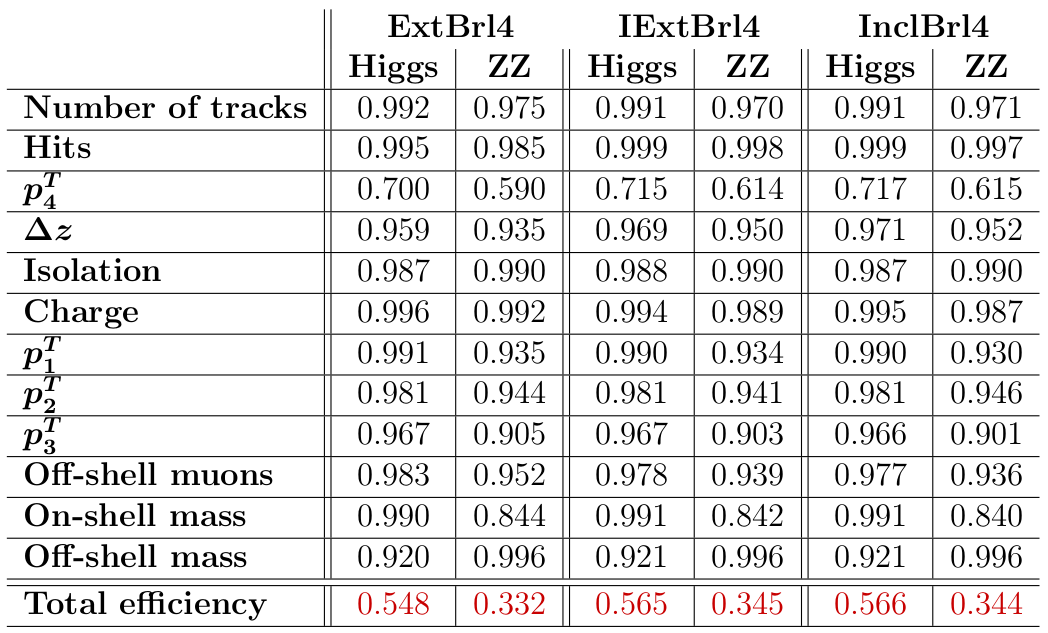
\includegraphics[width=\textwidth]{Efficiency}
\end{frame}

%----------------------------------------------

\begin{frame}[t]
\frametitle{Comparison with the Scoping Document}
\begin{columns}
\begin{column}{.6\textwidth}
\centering
Scoping Document: Efficiency
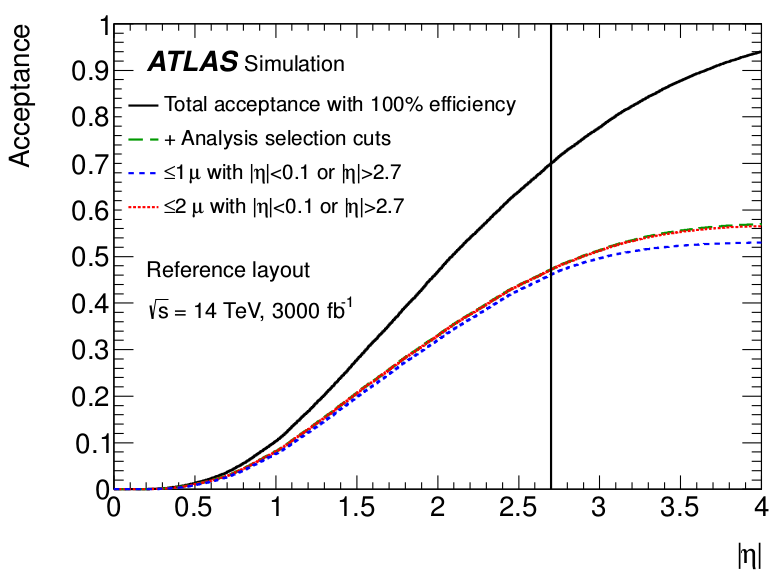
\includegraphics[width=\textwidth]{scopingAcceptance}
\end{column}
\begin{column}{.4\textwidth}
\resizebox{\textwidth}{!}{
\begin{tabular}{|c|c|c|}
\hline
 & \textbf{InclBrl4} & \textbf{Scoping} \\ \hline
\textbf{Geom. acc.} & 94.08\% & 94\% \\ \hline
\textbf{Total eff.} & 56.6\% & 57\% \\ \hline
\end{tabular}}
\end{column}
\end{columns}

\medskip
\begin{center}
\framebox{\color{dred} Very compatible results, but different layouts}
\end{center}
\end{frame}

%----------------------------------------------

\begin{frame}[t]
\frametitle{On-shell mass resolution}

\begin{columns}
\begin{column}{.5\textwidth}
\centering
\vskip1.2cm
Scoping Document
\includegraphics<1>[width=\textwidth,height=4.5cm]{scopingSigOnShell27}
\includegraphics<2>[width=\textwidth,height=4.5cm]{scopingSigOnShell32}
\includegraphics<3>[width=\textwidth,height=4.5cm]{scopingSigOnShell4}
\end{column}
\begin{column}{.5\textwidth}
\centering
\vskip0.6cm
Our analysis \\(InclBrl4 layout, no mass constraint)
\vskip0.1cm
\includegraphics<1>[width=\textwidth]{HZZ4mu/recoOnShellMass27}
\includegraphics<2>[width=\textwidth]{HZZ4mu/recoOnShellMass32}
\includegraphics<3>[width=\textwidth]{HZZ4mu/recoOnShellMass4}
\end{column}

\end{columns}
\end{frame}

%----------------------------------------------

\begin{frame}[t]
\frametitle{$4\mu$ mass resolution}

\begin{columns}
\begin{column}{.5\textwidth}
\centering
\vskip1.2cm
Scoping Document
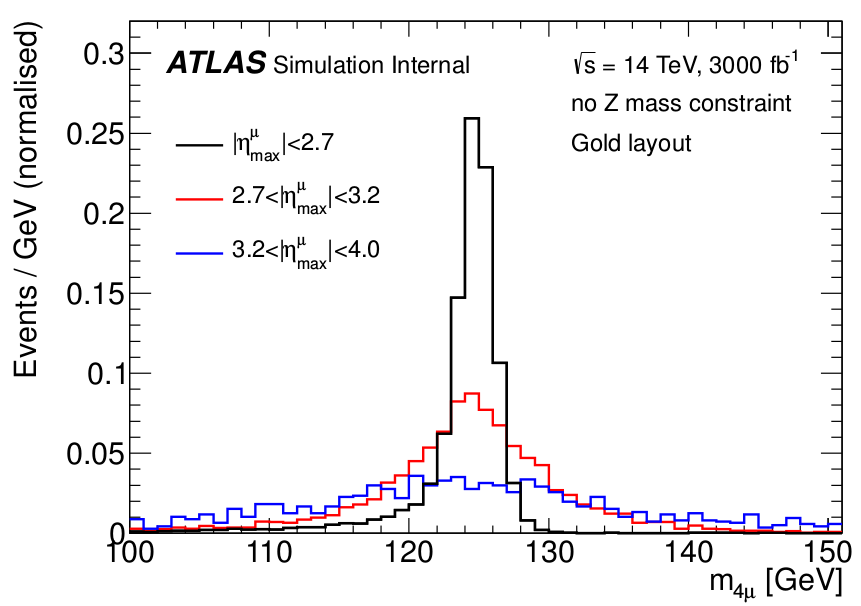
\includegraphics[width=\textwidth]{scopingRecoMass}
\end{column}
\begin{column}{.5\textwidth}
\centering
\vskip0.8cm
Our analysis \\(InclBrl4 layout, no mass constraint)
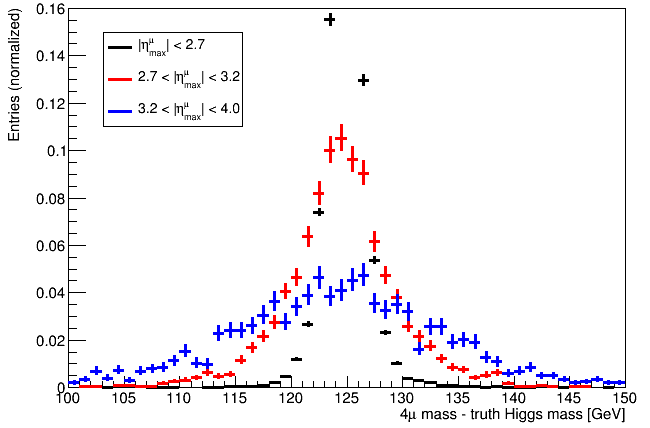
\includegraphics[width=\textwidth]{HZZ4mu/recoMass}
\end{column}

\end{columns}
\end{frame}

%----------------------------------------------

\begin{frame}
\frametitle{Higgs $p_{T}$, $\eta$, $\phi$ resolutions (InclBrl4 layout)}
\begin{columns}
\begin{column}{0.5\textwidth}
\centering
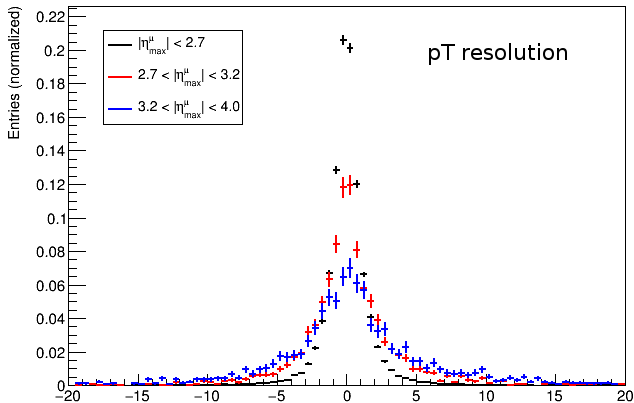
\includegraphics[width=\textwidth,height=3.7cm]{HZZ4mu/sigRecoPt}
\end{column}
\begin{column}{0.5\textwidth}
\centering
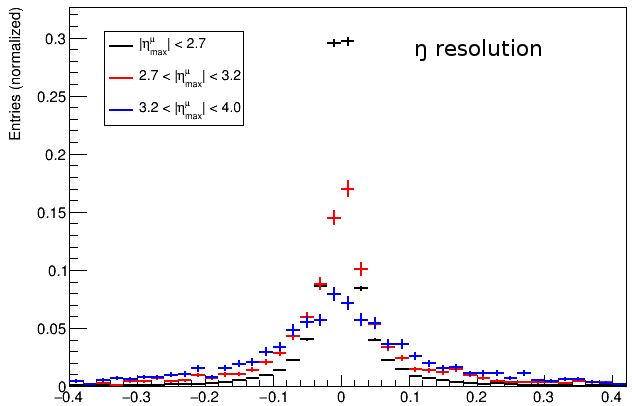
\includegraphics[width=\textwidth,height=3.7cm]{HZZ4mu/sigRecoEta}
\end{column}
\end{columns}
\vskip-0.5cm
\begin{center}
\centering
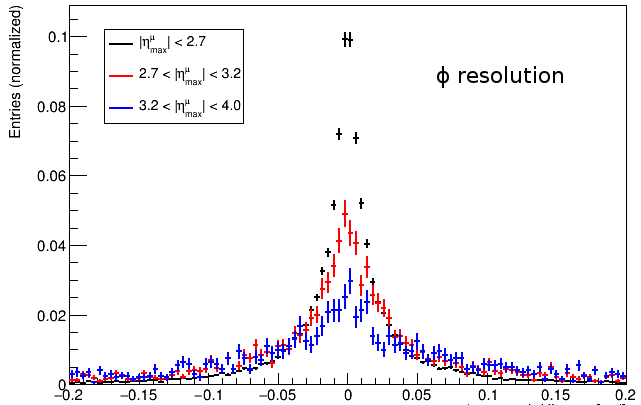
\includegraphics[width=0.5\textwidth,height=3.7cm]{HZZ4mu/sigRecoPhi}
\end{center}

\end{frame}


%----------------------------------------------

\begin{frame}
\frametitle{Muon $p_{T}$, $\eta$, $\phi$ resolutions}
\begin{columns}
\begin{column}{0.5\textwidth}
\centering
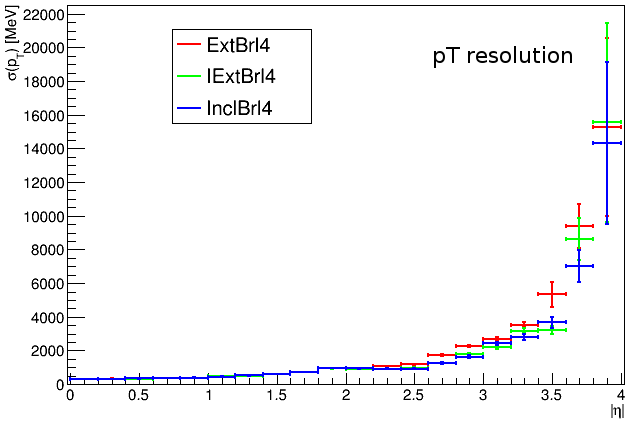
\includegraphics[width=\textwidth,height=3.7cm]{sigPt}
\end{column}
\begin{column}{0.5\textwidth}
\centering
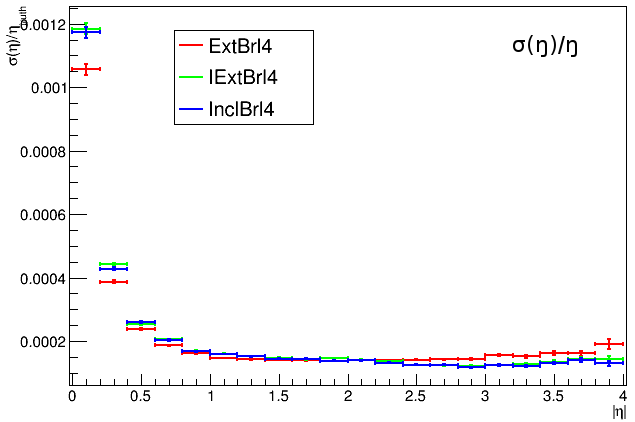
\includegraphics[width=\textwidth,height=3.7cm]{sigEta}
\end{column}
\end{columns}
\vskip-0.5cm
\begin{center}
\centering
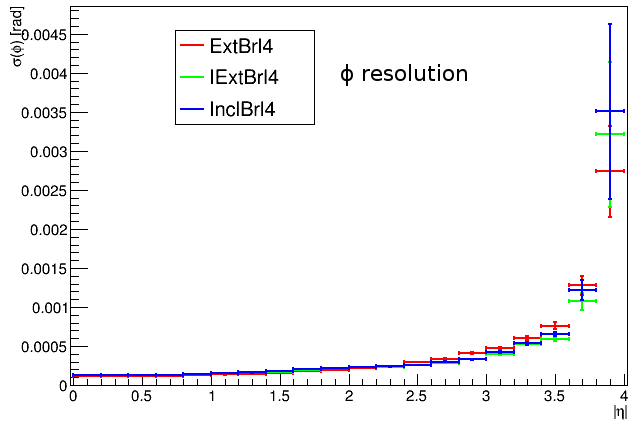
\includegraphics[width=0.5\textwidth,height=3.7cm]{sigPhi}
\end{center}

\end{frame}

%----------------------------------------------

\begin{frame}
\frametitle{Mass resolution - summary}
\centering

\begin{tikzpicture}
    \node[anchor=south west,inner sep=0] at (0,0) {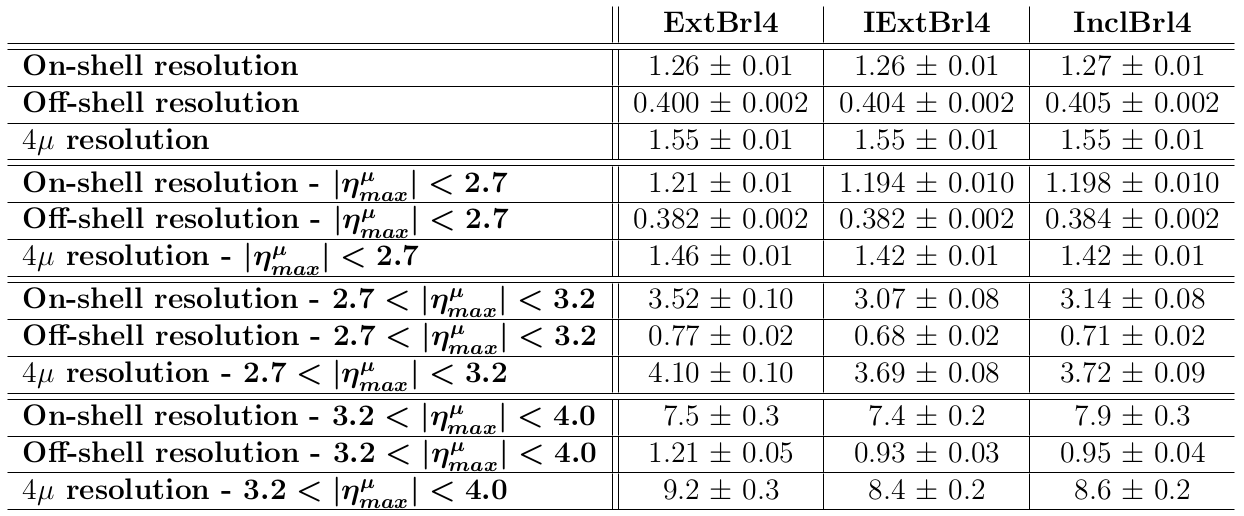
\includegraphics[width=\textwidth]{HZZ4mu/massResolutions}};
    \draw<2->[red,thick] (0.1,2.31) rectangle (12,2.67);
    \draw<2->[red,thick] (0.1,1.17) rectangle (12,1.57);
    \draw<2->[red,thick] (0.1,0.05) rectangle (12,0.42);
\end{tikzpicture}

\onslide<2->{
\begin{columns}
\begin{column}{.7\textwidth}
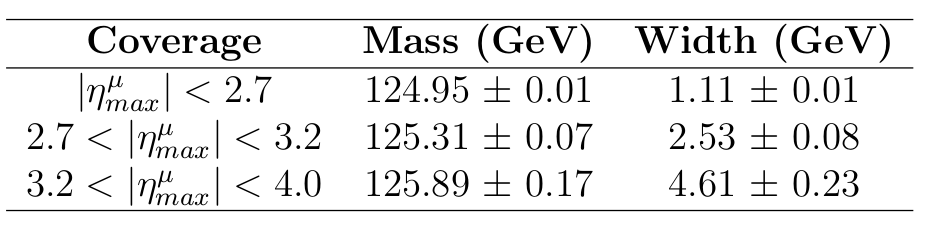
\includegraphics[width=\textwidth]{scopingResolution}
\end{column}
\begin{column}{.3\textwidth}
\textbf{Scoping Document}: \\
Better resolutions but Z mass constraint
\end{column}
\end{columns}}

\end{frame}

%----------------------------------------------

\begin{frame}
\frametitle{$p_T$, $\eta$, $\phi$ resolutions - summary}
\centering
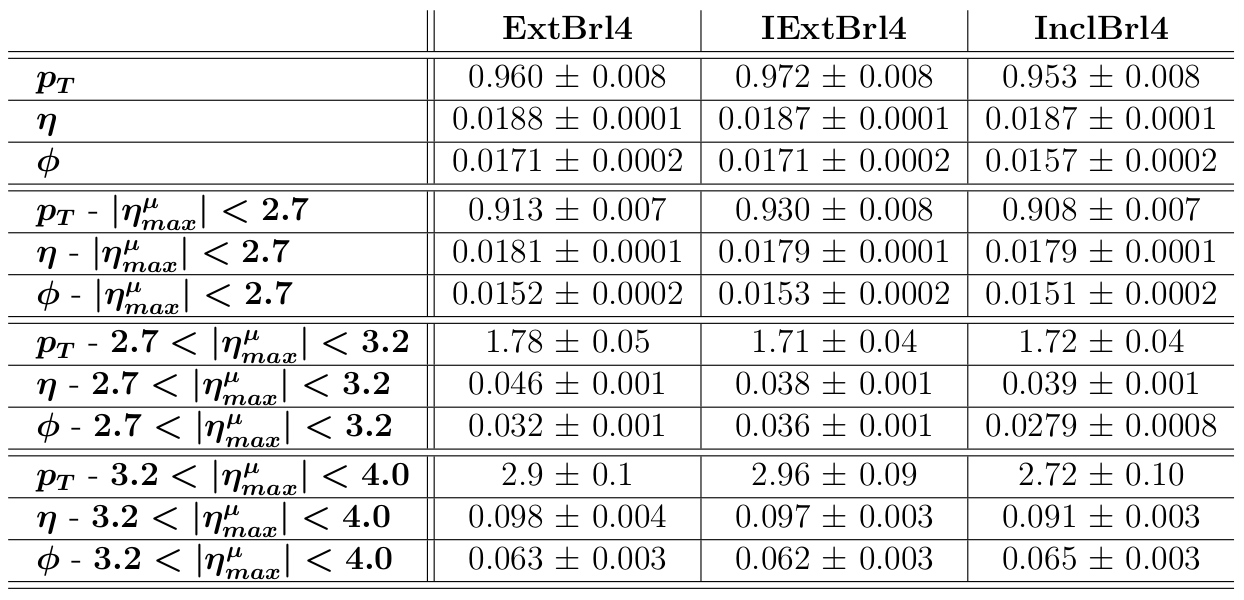
\includegraphics[width=\textwidth]{HZZ4mu/ptResolutions}
\end{frame}

%----------------------------------------------

\begin{frame}[t]
\frametitle{Channel significance}
\begin{center}
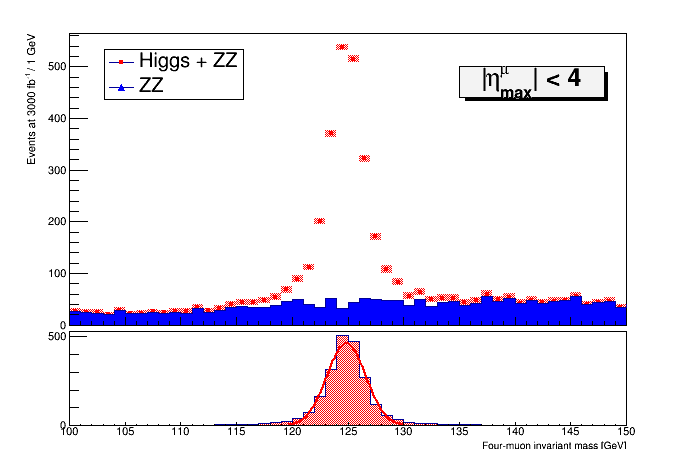
\includegraphics[width=.5\textwidth]{SBInclBrl4}
\end{center}

\begin{itemize}
\item Signal/background defined in [peak - 1.5$\sigma$, peak + 1.5$\sigma$]
\item Significance = $\frac{S}{\sqrt{S + B}}$
\item $\mu$ = $\frac{(\sigma \times BR)_{meas}}{(\sigma \times BR)_{SM}}$ $\rightarrow 
\Delta\mu/\mu \simeq \frac{\sqrt{S + B}}{S}$ (stat. only)
\end{itemize}
\end{frame}

%----------------------------------------------

\begin{frame}
\frametitle{Channel significance - summary}
\centering
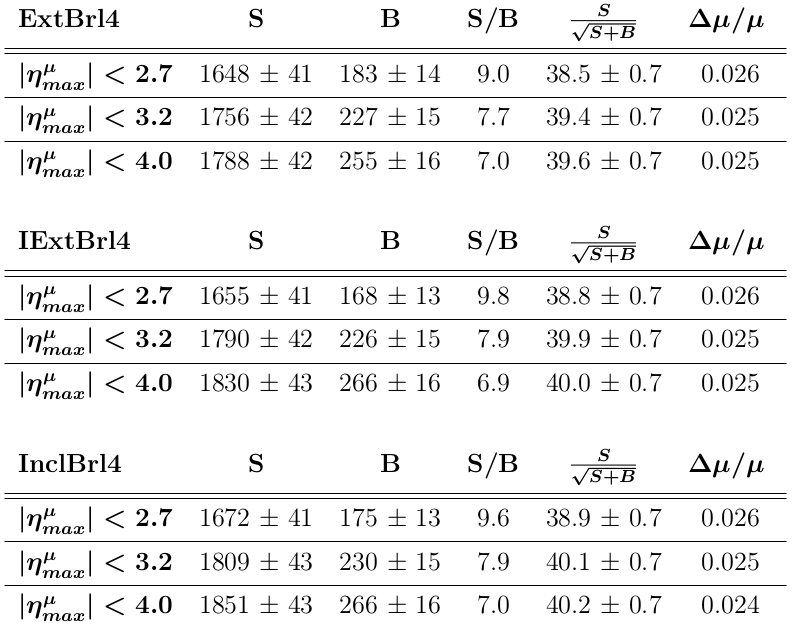
\includegraphics[width=.9\textwidth, height=7.5cm]{significance}
\end{frame}

%----------------------------------------------
\begin{frame}[t]
\frametitle{Channel significance - Scoping}

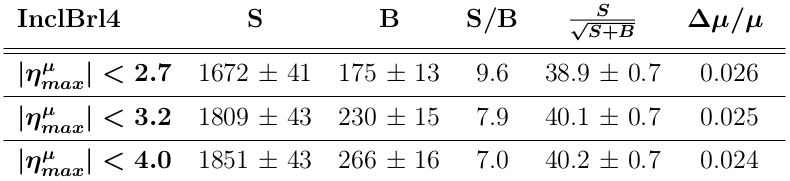
\includegraphics[width=.8\textwidth]{significanceInclBrl4}

\bigskip

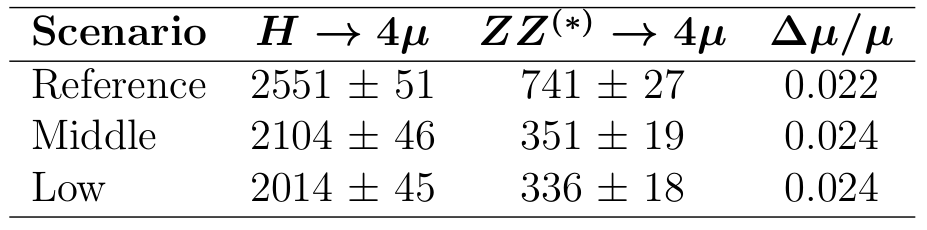
\includegraphics[width=.6\textwidth]{scopingSignificance}

\onslide<2->{
Differences:\\
\begin{itemize}
\item Scoping analysis is \textbf{inclusive} (factor 1.16 in $\sigma$)
\item Scoping analysis at 14 TeV, ours at 13 TeV (factor 1.13 in $\sigma$)
\item Generation selection of the final state radiation (factor 1.25)
\item Z mass constraint
\end{itemize}}
\end{frame}

%----------------------------------------------

\begin{frame}
\frametitle{Conclusions}
\begin{itemize}
\item<1-> We extended Soshi's fast simulation technique to physics samples
\item<2-> Step-1 layouts are robust against pile-up
\item<3-> We measured the $H \rightarrow 4\mu$ channel with a S/B of \textbf{at least} 7 and
a $\Delta\mu/\mu \sim$ 2.5\%, without considering the luminosity uncertainty \mbox{($\sim$ 3\%)}
\item<4-> The inclined layouts show slightly better performances, but the reconstruction
algorithm in the ExtBrl4 layout is not 
optimized in the forward region at Step-1 (long clusters)
\end{itemize}

\onslide<5->{
So:\\
\setbeamercolor{local structure}{fg=dred} 
\begin{itemize}
\item<5-> Early to draw conclusions but still a useful exercise that shows that the Step-1 layouts are
robust against pile-up also and respect the requirements for the $H \rightarrow 4\mu$ channel
\item<6-> The $\eta$ coverage extension to 3.2 provides measurements with better 
statistics, slight improvement with 4.0

\end{itemize}}
\end{frame}

%----------------------------------------------


%\begin{frame}
%\centering
%\huge \color{dred} \textbf{Backup slides}
%\end{frame}



\end{document}